\subsection{Adding External Knowledge}
\label{sec:wiki}

% All of the wikipedia inclusion work.

Note that phrases gain importance because of both their role in a
document but also from their semantic meaning in the broader world.
Variants of our next algorithms therefore integrate Wikipedia as a
knowledge source.

\subsubsection{Boosting Documents}

The first variant concatenates to each lecture a closely related
Wikipedia page, and then uses the techniques of
Section~\ref{sec:useTime} to choose phrases for the index. For
example, lecture title ``View Modifications Using Triggers'', yields
as the first Wikipedia result a page titled ``Database trigger.''
This page is appended to the lecture transcript. Using either
n-grams or adjective-noun phrases as candidate keywords, the algorithm
chooses phrases with TF-IDF over the combined document for the index.

\begin{figure}
\caption{The Document Boosting algorithm searches for a Wikipedia page using the title of the lecture, concatenates the result to the lecture, and then runs TF-IDF over the combined document.}
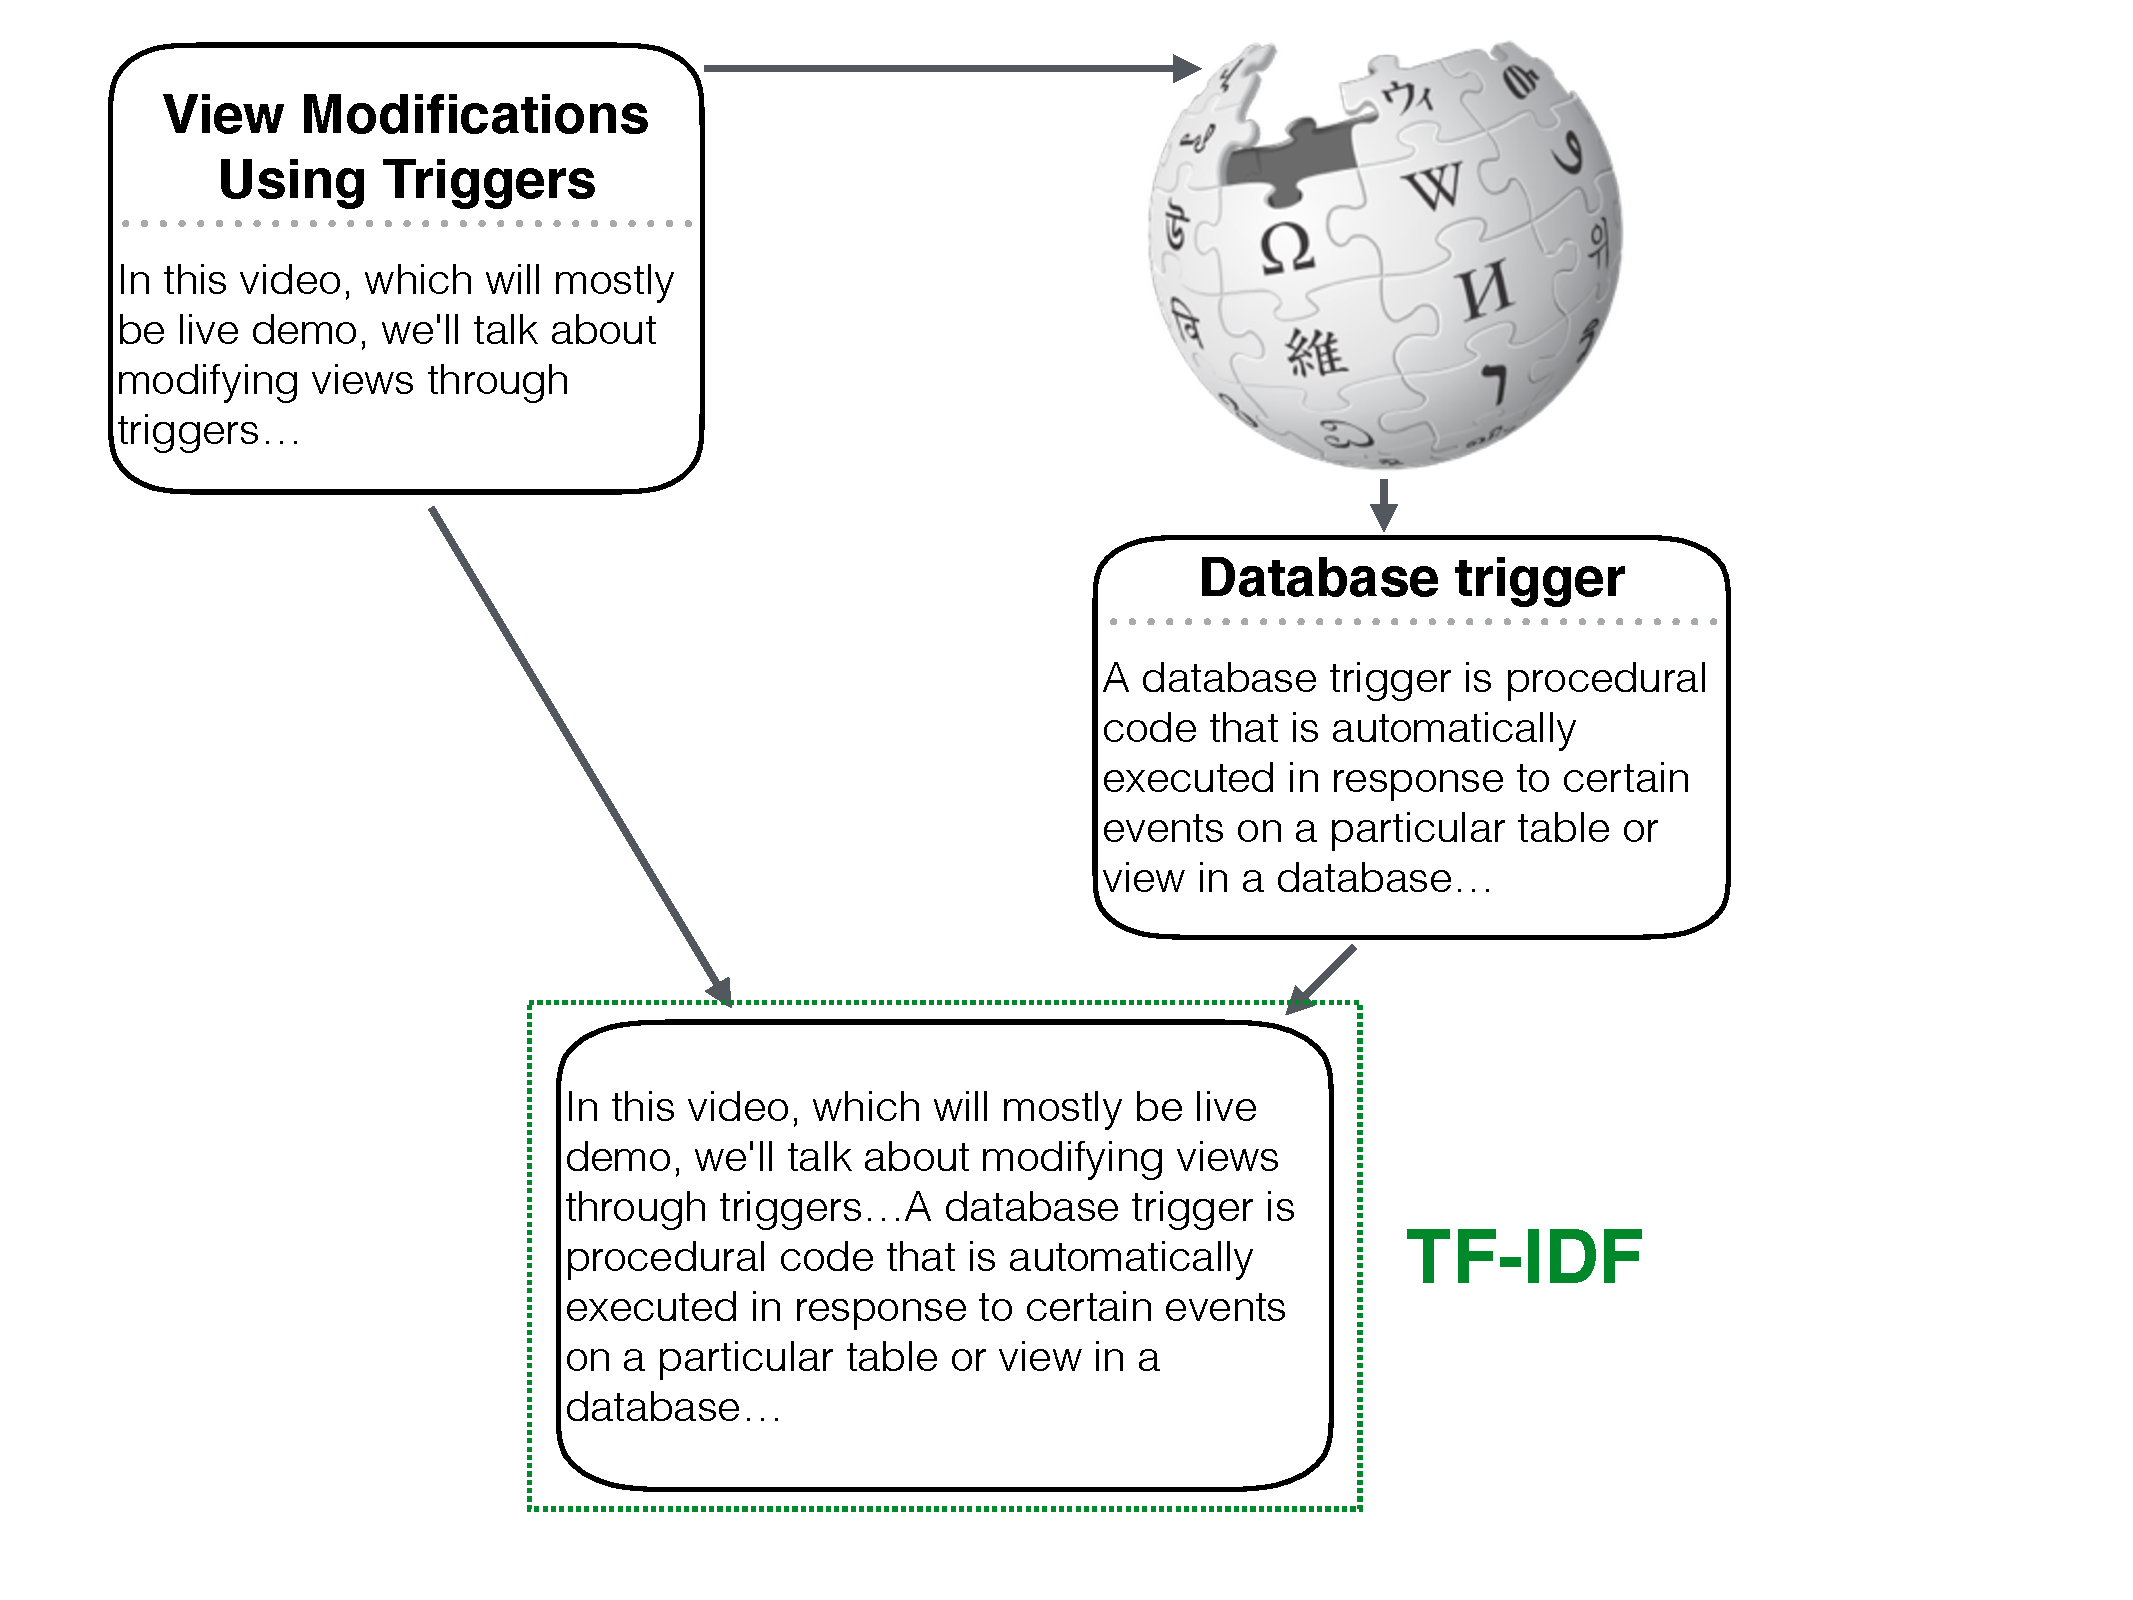
\includegraphics[width=\textwidth]{document_boosting.pdf}
\end{figure}

\subsubsection{Boosting Phrases}

This algorithm first creates a list of candidate index terms using
adjective-noun phrases. These candidates are ranked by their TF-IDF score
summed over {\bf all} Wikipedia documents.

Next, this global candidate ranking is combined with a basic TF-IDF
approach to form a final score that combines global knowledge (from
Wikipedia) with local knowledge (from the specific lecture video).
%
% First, we create a normalized Wikipedia candidate ranking
% \begin{equation*}
% TF\text{-}IDF_{w-norm}(p, W) \coloneqq \frac{TF\text{-}IDF_w(p, W)}{\sum_{p'} TF\text{-}IDF_w(p', W)}
% \end{equation*}
% and normalized lecture collection ranking
% \begin{equation*}
% TF\text{-}IDF_{norm}(p, l, L) \coloneqq \frac{TF\text{-}IDF(p, l, L)}{\sum_{p'} TF\text{-}IDF(p', l, L)}
% \end{equation*}
% Then, we combine the two normalized rankings to form a final score
% \begin{multline*}
% TF\text{-}IDF_{combined}(p, l, L, W) \coloneqq \\ \eta TF\text{-}IDF_{w-norm}(p, W) + TF\text{-}IDF_{norm}(p, l, L)
% \end{multline*}
% where $\eta$ is used to determine the weight between Wikipedia scores
% and lecture scores.

We also experimented with only boosting phrases of at least two words,
based on the intution that longer phrases are often meaningful, but
appear infrequently and are therefore given low scores by TF-IDF. We
call this alternative ``Phrase Boosting N-Grams'' in Figure
\ref{fig:main_result}.

\begin{figure}[!htbp]
\caption{The top 15 keywords from `Materialized Views' by Phrase
  Boosting with N-grams. Phrases that also appear in the gold index are marked in bold.}
\label{fig:top_15}
\begin{tabular}{|l|l|}
\hline
Rank & Phrase \\
\hline
1 & \textbf{view} \\
\hline
2 & \textbf{materialized view} \\
\hline
3 & materialized \\
\hline
4 & \textbf{query} \\
\hline
5 & \textbf{view query} \\
\hline
6 & \textbf{virtual view} \\
\hline
7 & \textbf{modify} \\
\hline
8 & user query \\
\hline
9 & \textbf{base table} \\
\hline
10 & \textbf{modify command} \\
\hline
11 & \textbf{index} \\
\hline
12 & insert command \\
\hline
13 & multivalued dependency \\
\hline
14 & \textbf{database design} \\
\hline
15 & user \\
\hline
\end{tabular}
\end{figure}

%
% A few subtleties deserve further description. First, in our simple
% TF-IDF approach, a score is calculated for each lecture $l$ and phrase
% $p$, while in our Wikipedia calculation a score is only calculated for
% each $p$. That approach is chosen because in this algorithm we are not interested in
% keywords for every Wikipedia document, but only in obtaining a global sense
% of the importance of a phrase. The algorithm is equivalent to summing over all
% Wikipedia documents $d \in W$
% \begin{equation*}
% TF_w(p) = \log \left(\sum_{d \in W} \text{number of times } p \text{ appears in } d\right)
% \end{equation*}
%
% Second, we take the logarithm of the phrase count in the Wikipedia
% ranking. This choice produces improved empirical results.
%
% \begin{figure}
% \caption{The Phrase Boosting algorithm runs TF-IDF over the entirety of Wikipedia and then combines the global ranking with a local ranking for a document.}
% 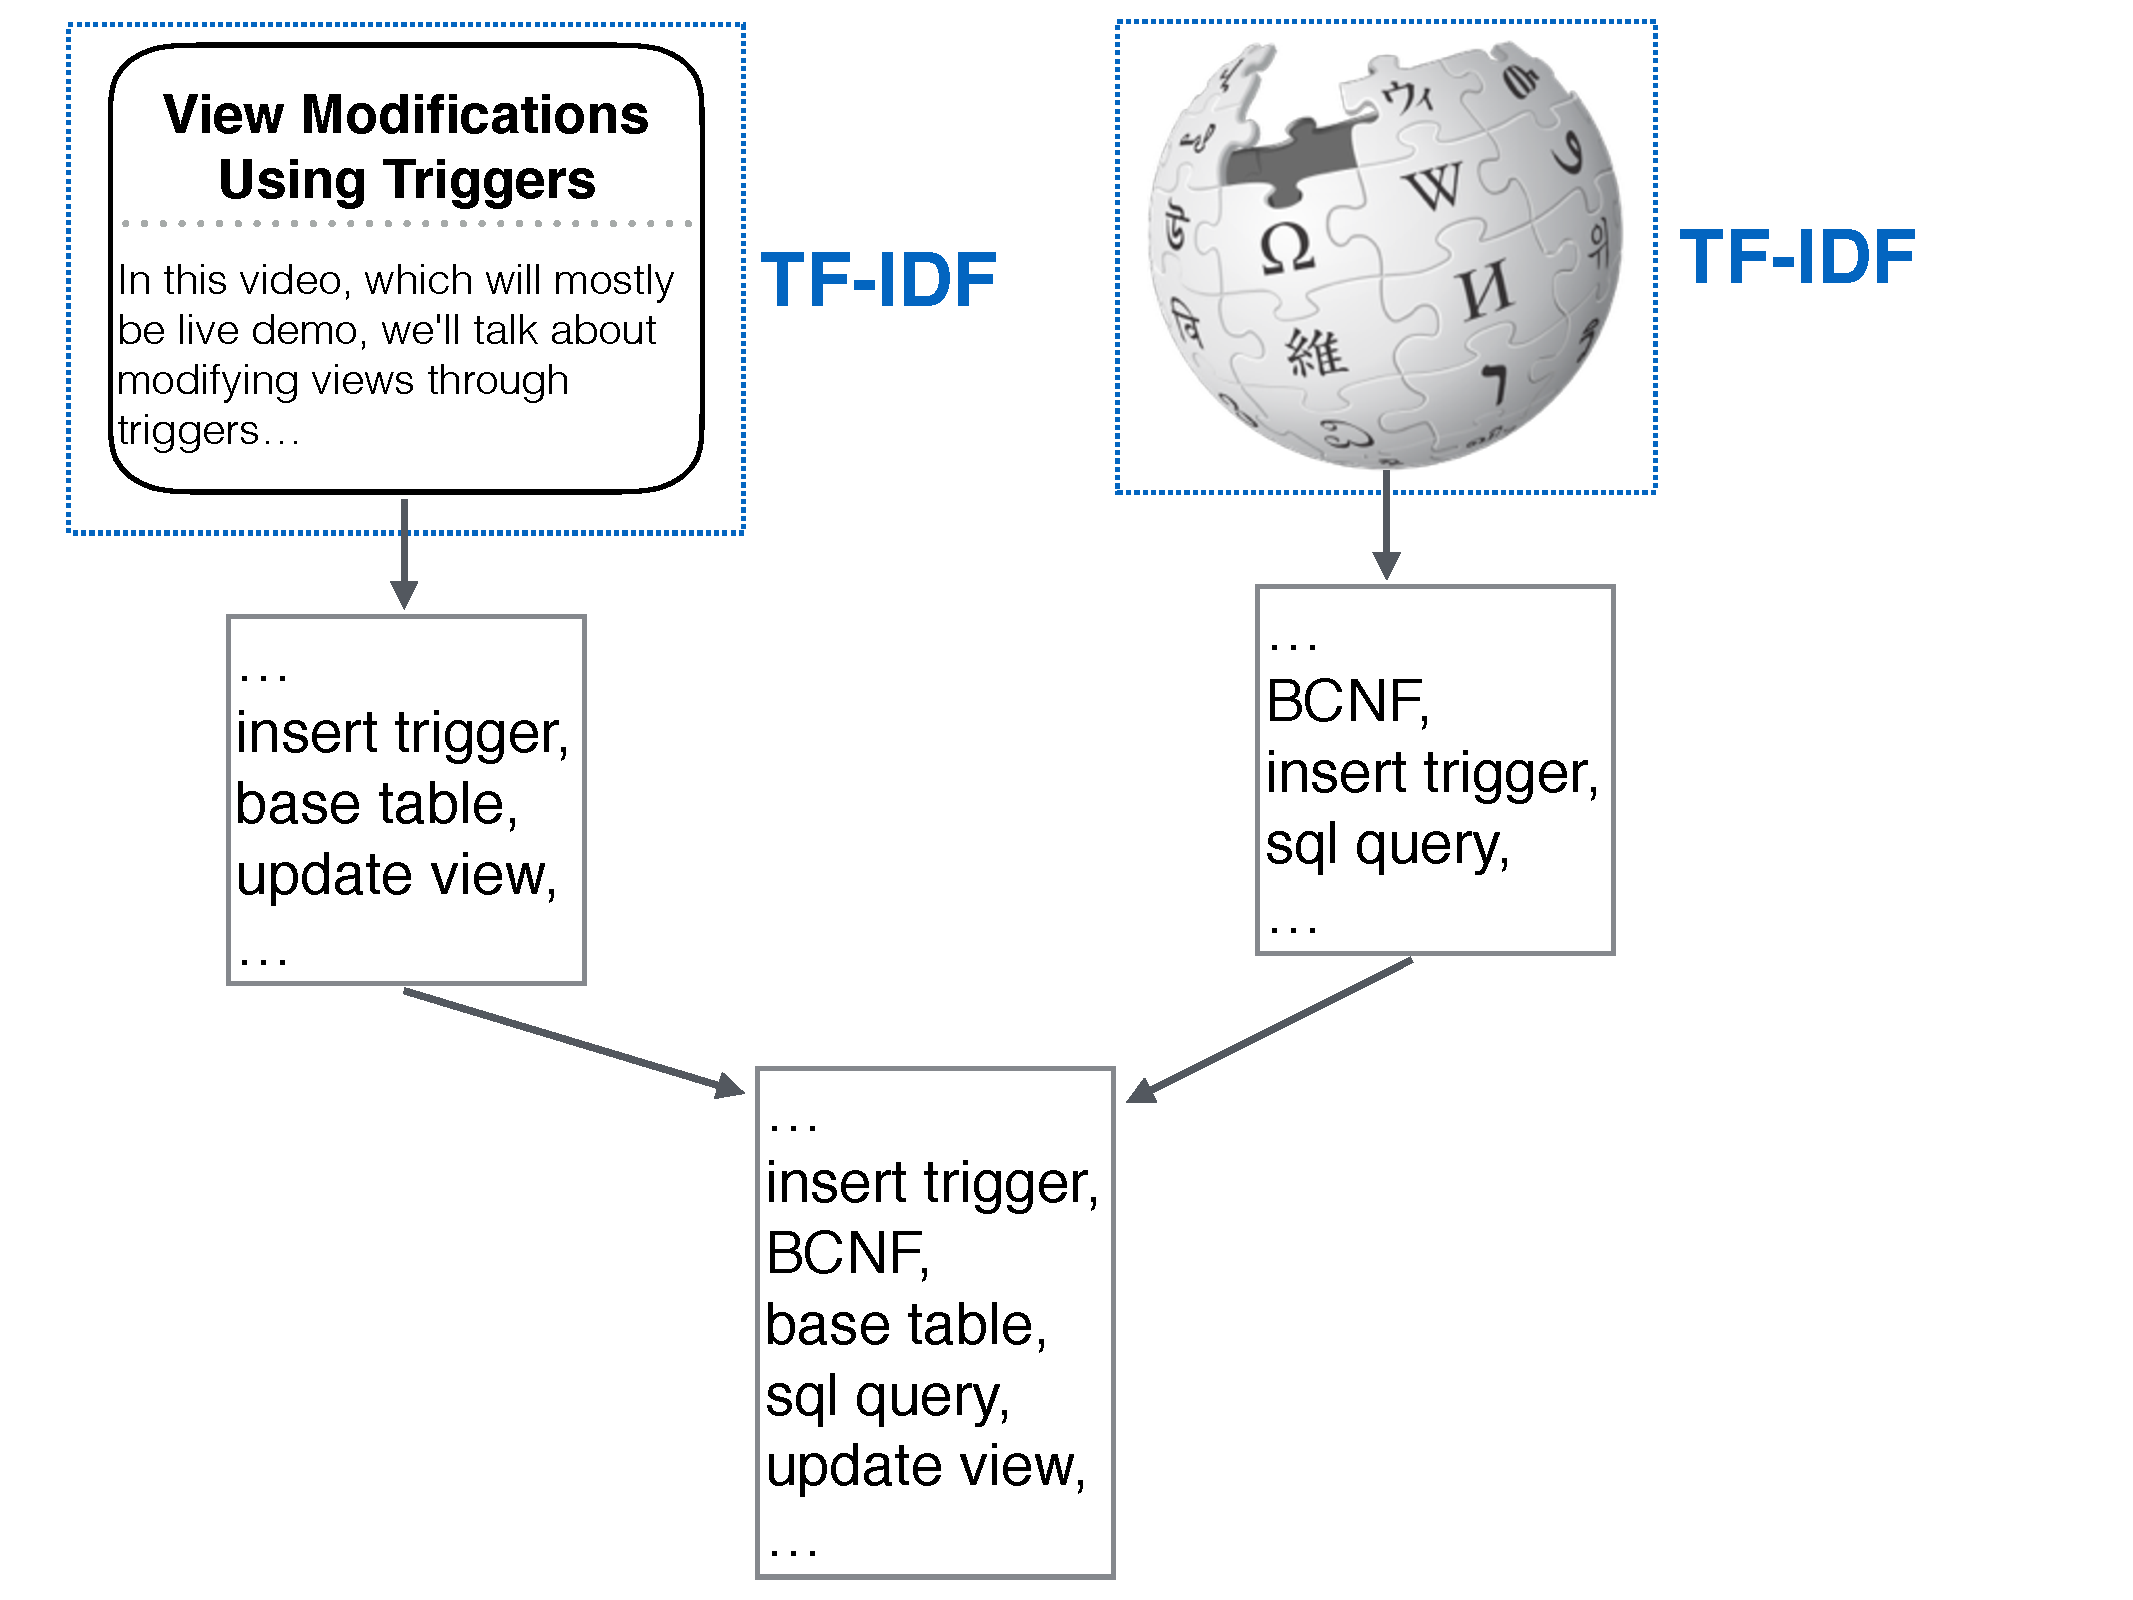
\includegraphics[width=\textwidth]{phrase_boosting.pdf}
% \end{figure}
